\chapter{Generator Peeling}
\label{chp:ch4-peeling}

Generators offer an elegant way to express iterators.
However, performance has always been their Achilles heel and has prevented widespread adoption.
We present techniques to efficiently implement and optimize generators.

We have implemented our optimizations in ZipPy, a modern, light-weight AST interpreter based Python 3 implementation targeting the Java virtual machine.
Our implementation builds on a framework that optimizes AST interpreters using just-in-time compilation.
In such a system, it is crucial that AST optimizations do not prevent subsequent optimizations.
Our system was carefully designed to avoid this problem.
We report an average speedup of \peelingSpeedup{}$\times$ for generator-bound programs.
As a result, using generators no longer has downsides and programmers are free to enjoy their upsides.

\section{Motivation}

Many programming languages support generators, which allow a natural expression of iterators.
We surveyed the use of generators in real Python programs, and found that among the 50 most popular Python projects
listed on the Python Package Index (PyPI)~\cite{pypi} and GitHub~\cite{github}, 90\% of these programs use generators.

Generators provide programmers with special control-flow transfers that allows function executions to be suspended and resumed.
Even though these control-flow transfers require extra computation, the biggest performance bottleneck is caused by preserving the state of a function between a suspend and a resume.
This bottleneck is due to the use of \emph{cactus} stacks required for state preservation.
Popular language implementations, such as CPython~\cite{python}, and CRuby~\cite{ruby}, allocate frames on the heap.
Heap allocation eliminates the need for cactus stacks, but is expensive on its own.
Furthermore, function calls in those languages are known to be expensive as well.

In this thesis, we examine the challenges of improving generator performance for Python.
First, we show how to efficiently implement generators in abstract syntax tree (AST) interpreters,
which requires a fundamentally different design than existing implementations for bytecode interpreters.
We use our own full-fledged prototype implementation of Python 3, called ZipPy\footnote{Publicly available at \url{https://bitbucket.org/ssllab/zippy}},
which targets the Java virtual machine (JVM).
ZipPy uses the Truffle framework~\cite{Wurthinger+13} to optimize interpreted programs in stages, first collecting type feedback in the AST interpreter,
then just-in-time compiling an AST down to optimized machine code.
In particular, our implementation takes care not to prevent those subsequent optimizations.
Our efficient generator implementation optimizes control-transfers via suspend and resume.

Second, we describe an optimization for frequently used idiomatic patterns of generator usage in Python.
Using this optimization allows our system to allocate generator frames to the native machine stack, eliminating the need for heap allocation.
When combined, these two optimizations address both bottlenecks of using generators in popular programming languages, and finally give way to high performance generators.

\noindent{}Summing up, our contributions are:

\begin{itemize}
\item We present an efficient implementation of generators for AST based interpreters that is easy to implement and enables efficient optimization offered by just-in-time compilation.
\item We introduce \emph{generator peeling}, a new optimization that eliminates overheads incurred by generators.
\end{itemize}

\section{Generators in Python}

A generator is a more restricted variation of a coroutine~\cite{grune1977view,Moura2009}.
It encompasses two control abstractions: \emph{suspend} and \emph{resume}.
\emph{Suspend} is a generator exclusive operation, while only the caller of a generator can \emph{resume} it.
Suspending a generator always returns control to its immediate caller.
Unlike regular subroutine calls, which start executing at the beginning of the callee, calls to a \emph{suspended} generator resume
from the point where it most recently suspended itself.
Those two operations are asymmetric as opposed to the symmetric control \emph{transfer} in coroutines.

\subsubsection*{Generator Functions}

\begin{figure}
\centering
\subfigure[Simple generator]{
	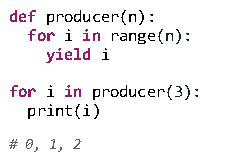
\includegraphics[scale=1.5]{figures/ch4-simple-generator-example-code}
	\label{fig:ch4-simple-generator-code}
}
\subfigure[Python iterator protocol]{
	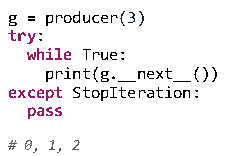
\includegraphics[scale=1.5]{figures/ch4-loop-on-generator-code}
	\label{fig:ch4-iterate-on-generator-code}
}
\caption{A simple generator function in Python}
\label{fig:ch4-generator-example}
\end{figure}

In Python, using the \texttt{yield} keyword in a function definition makes the function a generator function.
A call to a generator function returns a generator object without evaluating the body of the function.
The returned generator holds an execution state initialized using the arguments passed to the call.
Generators implement Python's iterator protocol, which includes a \texttt{\_\_next\_\_} method.
The \texttt{\_\_next\_\_} method starts or resumes the execution of a generator.
It is usually called implicitly, e.g., by a for loop that iterates on the generator (see Figure~\ref{fig:ch4-simple-generator-code}).
When the execution reaches a \texttt{return} statement or the end of the generator function, the generator raises a \texttt{StopIteration} exception.
The exception terminates generator execution and breaks out of the loop that iterates on the generator.
Figure~\ref{fig:ch4-iterate-on-generator-code} shows the desugared version of the for loop that iterates over the generator object \texttt{g} by explicitly calling \texttt{\_\_next\_\_}.

\subsubsection*{Generator Expressions}

\begin{figure}[h]
\centering
\subfigure[Generator expression]{
	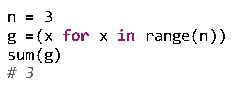
\includegraphics[scale=1.5]{figures/ch4-genexp-example-code}
	\label{fig:ch4-simple-genexp-code}
}
\subfigure[Desugared generator function]{
	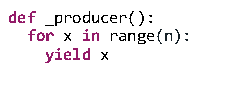
\includegraphics[scale=1.5]{figures/ch4-genexp-desugared-code}
	\label{fig:ch4-genexp-desugared-code}
}
\caption{A simple generator expression in Python}
\label{fig:ch4-genexp-example}
\end{figure}

Generator expressions offer compact definitions of simple generators in Python.
Generator expressions are as memory efficient as generator functions, since they both create generators that lazily produce one element at a time.
Programmers use these expressions in their immediate enclosing scopes.
Figure~\ref{fig:ch4-genexp-example} shows a simple generator expression and its equivalent, desugared generator function definition.
A generator expression defines an anonymous generator function, and directly returns a generator that uses the anonymous function definition.
The returned generator encapsulates its enclosing scope, if the generator expression references symbols in the enclosing scope (\texttt{n} in Figure~\ref{fig:ch4-genexp-example}).
The function \texttt{sum} subsequently consumes the generator by iterating on it in a loop and accumulating the values produced by the generator.

\subsubsection*{Idiomatic Uses of Generators}

\begin{figure}[h]
\centering
\subfigure[Generator loop]{
	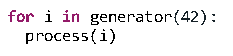
\includegraphics[scale=1.5]{figures/ch4-idiomatic-generator-loop-code}
	\label{fig:ch4-idiomatic-loop-code}
}
\subfigure[Implicit generator loop]{
	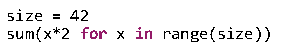
\includegraphics[scale=1.5]{figures/ch4-idiomatic-implicit-loop-code}
	\label{fig:ch4-idiomatic-implicit-code}
}
\caption{Idiomatic uses of generators}
\label{fig:ch4-idiomatic-patterns}
\end{figure}

The idiomatic way of using generators in Python is to write a \emph{generator loop}.
As shown in Figure~\ref{fig:ch4-idiomatic-loop-code}, a generator loop is a for loop that calls a generator function and consumes the returned generator object.
The common use pattern of a generator expression is to use it as a closure and pass it to a function that consumes it (see Figure~\ref{fig:ch4-idiomatic-implicit-code}).
The consumer functions, like \texttt{sum}, usually contain a loop that iterates on the generator.
Therefore, we refer to this pattern as an \emph{implicit generator loop}.
Explicit and implicit generator loops cover most of the generator usage in Python programs.
Our generator peeling optimization, which we explain in Section~\ref{sec:ch4-generaor-peeling}, targets these patterns.

\section{Generators Using an AST Interpreter}

Java, the host language of Truffle and ZipPy, does not offer native support for coroutines.
Our AST interpreter needs to model the semantics of generators.
However, the conventional way of implementing generators in a bytecode interpreter does not work in an AST setting.
In this section, we discuss the challenges of supporting generators in an AST interpreter, and present the solution we devised for ZipPy.

\subsection{AST Interpreters vs. Bytecode Interpreters}

\begin{figure}
\centering
\subfigure[Implementation of \texttt{WhileNode}]{
	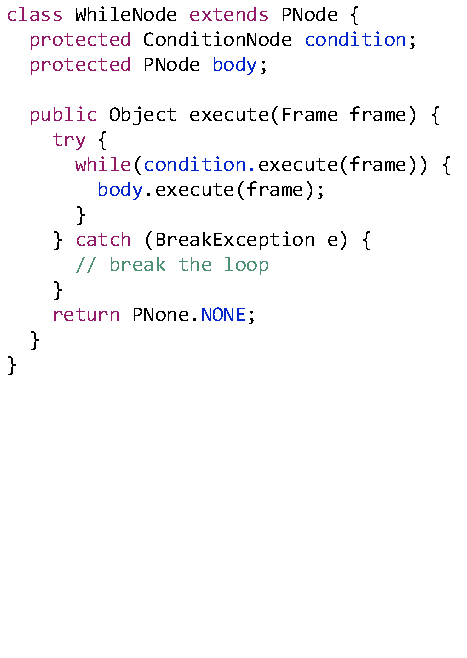
\includegraphics[scale=.9]{figures/ch4-while-node-code}
	\label{fig:ch4-while-node-code}
}
\subfigure[Implementation of \texttt{GenWhileNode}]{
	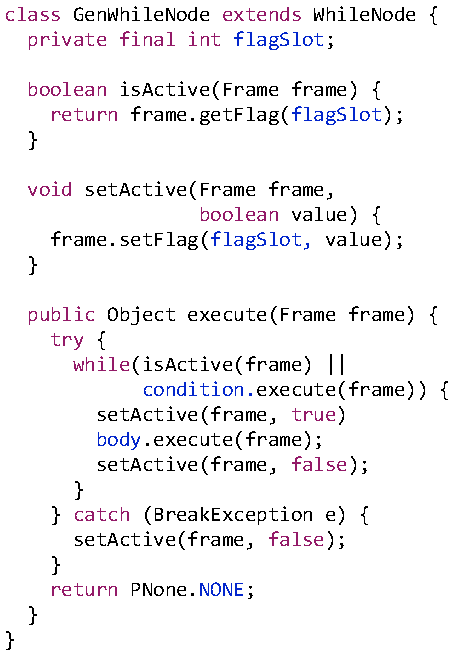
\includegraphics[scale=.9]{figures/ch4-gen-while-node-code}
	\label{fig:ch4-gen-while-node-code}
}
\caption{Two different \texttt{WhileNode} versions}
\label{fig:ch4-while-nodes}
\end{figure}

The de-facto Python implementation, CPython, uses bytecode interpretation.
It parses the Python program into a linearized bytecode representation and executes the program using a bytecode interpreter.
A bytecode interpreter is \emph{iterative}.
It contains an interpreter loop that fetches the next instruction in every iteration and performs its operation.
The bytecode index pointing to the next instruction is the only interpreter state that captures the current location of the program.
The interpreter only needs to store the program activation and the \emph{last} bytecode index when the generator suspends.
When resuming, a generator can simply load the program activation and the \emph{last} bytecode index before it continues with the next instruction.

An AST interpreter on the other hand is \emph{recursive}.
The program evaluation starts from the root node, then recursively descends to the leaves, and eventually returns to the root node.
In ZipPy, every AST node implements an \texttt{execute} method (see Figure~\ref{fig:ch4-while-nodes}).
Each \texttt{execute} method recursively calls the \texttt{execute} methods on its child nodes.
The recursive invocation builds a native call stack that captures the current location of the program.
The interpreter has to save the entire call stack when the generator suspends.
To resume the generator execution, it must rebuild the entire call stack to the exact point where it last suspended.

\subsection{Generator ASTs}
\label{sec:ch4-generator-ast}

ZipPy stores local variables in a heap-allocated frame object.
AST nodes access variables by reading from and writing to dedicated frame slots.
During just-in-time compilation, Truffle is able to map frame accesses to the machine stack and eliminate frame allocations.
However, a generator needs to store its execution state between a suspend and resume.
The frame object must therefore be kept on the heap which prevents Truffle's frame optimization.

In general, our AST interpreter implements control structures using Java's control structures.
We handle non-local returns, i.e., control flow from a deeply nested node to an outer node in the AST, using Java exceptions.
Figure~\ref{fig:ch4-genfunc-before} illustrates the AST of a Python generator function.
We model loops or if statements using dedicated \emph{control nodes}, e.g., a \texttt{WhileNode}.
The \texttt{BlockNode} groups a sequence of nodes that represents a basic block.
The \texttt{YieldNode} performs a non-local return by throwing a \texttt{YieldException}.
The exception bypasses the two parent \texttt{BlockNode}s, before the \texttt{FunctionRootNode} catches it.
The \texttt{FunctionRootNode} then returns execution to the caller.

\subsubsection*{Generator Control Nodes}

\begin{figure}
\centering
\subfigure[Before translation]{
	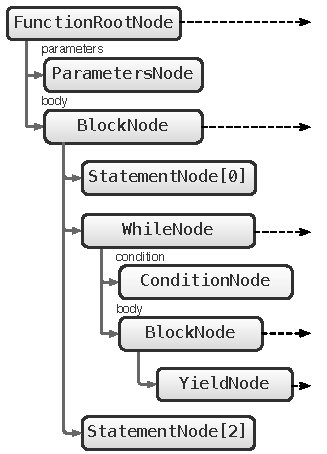
\includegraphics[scale=1.1]{figures/ch4-gen-function-orig}
	\label{fig:ch4-genfunc-before}
}
\subfigure[Translated]{
	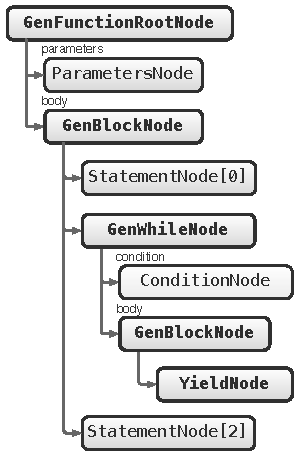
\includegraphics[scale=1.1]{figures/ch4-gen-function-translated}
	\label{fig:ch4-genfunc-translated}
}
\caption{Translation to generator AST}
\label{fig:ch4-genfunc-translation}
\end{figure}

Every control node in ZipPy has a local state stored in the local variables of its \texttt{execute} method.
The local state captures the current execution of the program, for instance, the current iterator of a for loop node or the current node index of a block node.
To support generators we decide to implement an alternative generator version for each control node.
These control nodes do not rely on local state, and keep all execution state in the frame.
However, it is overly conservative to use generator control nodes everywhere in a generator function.
We only need to use generator control nodes for the parent nodes of \texttt{YieldNode}s, since a yield operation only suspends the execution of these nodes.

Figure~\ref{fig:ch4-while-node-code} shows the implementation of a \texttt{WhileNode}.
Note that the loop condition result is a local state of the node stored in the call stack of its \texttt{execute} method.
When a \texttt{YieldException} is thrown somewhere in the loop body, it unwinds the call stack and discards the current loop condition result.
When the generator resumes, it will not be able to retrieve the previous loop condition result without re-evaluating the \texttt{condition} node.
The re-evaluation may have side effects and violate correct program behavior.
Therefore, this implementation only works for normal functions but not for generator functions.

Figure~\ref{fig:ch4-gen-while-node-code} shows the generator version of the \texttt{WhileNode}, the \texttt{GenWhileNode}.
It keeps an \emph{active} flag, a local helper variable, in the frame.
The \texttt{execute} method accesses the flag by calling the \texttt{isActive} or \texttt{setActive} method.
When a yield occurs in the loop body, the active flag remains true.
When resuming, it bypasses the condition evaluation and forwards execution directly to the loop body.

Note that it is incorrect to store the active flag as a field in the \texttt{GenWhileNode}.
Different invocations of the same generator function interpret the same AST, but should not share any state stored in the AST.
An alternative way to implement a \texttt{GenWhileNode} is to catch \texttt{YieldException}s in the \texttt{execute} method and set the active flag in the catch clause.
This implementation requires the \texttt{GenWhileNode} to re-throw the \texttt{YieldException} after catching it.
If we implement generator control nodes in this way, a yield operation will cause a chain of Java exception handling which is more expensive than the solution we chose.

Similar to the \texttt{GenWhileNode}, we implement a generator version for all the other control nodes in ZipPy.
Every generator control node has its own active flags stored in the frame.
The descriptions of the generator control nodes are as follows:

\begin{itemize}

\item \texttt{GenFunctionRootNode}:
Stores an active flag in the frame.
Only applies arguments when the flag is false.
Resets the flag and throws \texttt{StopIteration} exception upon termination of the generator.

\item \texttt{GenBlockNode}:
Stores the current node index in the frame.
Skips the executed nodes when the index is not zero.
Resets the index to zero upon exit.

\item \texttt{GenForNode}:
Stores the current iterator in the frame.
Resets the iterator to \texttt{null} upon exit.

\item \texttt{GenIfNode}:
Similar to \texttt{GenWhileNode}, uses an active flags to indicate which branch is active.

\item \texttt{GenWhileNode}:
See Figure~\ref{fig:ch4-gen-while-node-code}.

\item \texttt{GenBreakNode}:
Resets active flags of the parent control nodes up to the targeting loop node (the innermost enclosing loop), including the loop node.

\item \texttt{GenContinueNode}:
Resets active flags of the parent control nodes up to the targeting loop node, excluding the loop node.

\item \texttt{YieldNode}:
Must be a child of a \texttt{GenBlockNode}.
Evaluates and stores the yielding value in the frame before throwing the \texttt{YieldException}.
The root node then picks up the value and returns it to the caller.
The \texttt{YieldNode} also advances the statement index of its parent \texttt{BlockNode} to ensure that the generator resumes from the next statement.

\end{itemize}

\subsubsection*{Control Node Translation}
\label{sec:ch4-ast-of-gen-func}

ZipPy first parses Python functions into ASTs that use the \emph{normal} control nodes.
Generator functions require an additional translation phase that replaces the \emph{normal} control nodes with their \emph{generator} equivalents.
Figure~\ref{fig:ch4-genfunc-translation} illustrates this translation.
We only replace the control nodes that are parents of the \texttt{YieldNode}s, since these nodes fully capture the state required to suspend and resume execution.

The translated generator AST always keeps a snapshot of its execution in the frame.
When resuming, it is able to retrieve all the necessary information from the snapshot and rebuild the entire interpreter call stack to the exact point where it left off.

The flag accesses in the generator control nodes and the exception based control flow handling add performance overheads.
However, the underlying compiler is able to compile the entire generator AST into machine code.
It also optimizes control flow exceptions and converts them to direct jumps.
The jumps originate from where the exception is thrown and end at the location that catches it.
The AST approach, enforced by the underlying framework, does add complexity to the implementation of generators.
However, the performance gains offset this slight increase of the implementation effort.

\subsubsection*{Yield as an Expression}

\begin{figure}[h]
\centering
\subfigure[Yield expression]{
	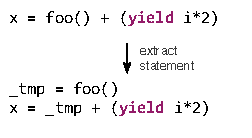
\includegraphics[scale=1.45]{figures/ch4-yield-expression-example}
	\label{fig:ch4-yield-expression-example}
}
\subfigure[Translated multiply]{
	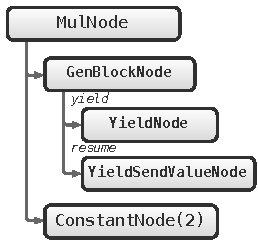
\includegraphics[scale=1.1]{figures/ch4-yield-expression-ast}
	\label{fig:ch4-yield-expression-ast}
}
\caption{Translation of a yield expression}
\label{fig:ch4-yield-expression}
\end{figure}

Python allows programmers to use yield in expressions.
A yield expression returns a value passed from the caller by calling the generator method \texttt{send}.
This enhancement allows the caller to pass a value back to the generator when it resumes, and brings generators closer to coroutines.
However, it requires generator ASTs to be able to resume to a specific expression.

Figure~\ref{fig:ch4-yield-expression-example} shows an example of yield expressions.
The assignment statement to variable \texttt{x} consumes the value returned by the yield expression.
Figure~\ref{fig:ch4-yield-expression-ast} shows the translated AST of the multiplication sub-expression.
Note that we translate the yield expression to a \texttt{GenBlockNode} containing a \texttt{YieldNode} and a \texttt{YieldSendValueNode}.
When the \texttt{YieldNode} suspends execution, it advances the active node index of the parent \texttt{GenBlockNode} to point to the next node.
This action ensures that the generator restarts execution from the \texttt{YieldSendValueNode}, which returns the value sent from the caller.

In a more complicated case, the statement consuming the yield expression could contain sub-expressions with a higher evaluation order.
In other words, the interpreter should evaluate these expressions before the yield expression.
Some of them could have side effects, i.e., the call to \texttt{foo} in Figure~\ref{fig:ch4-yield-expression-example}.
To avoid re-evaluation, we convert such expressions into separate statements and create variables to store the evaluated values.
When the generator resumes, it picks up the evaluated values from the variables without visiting the expression nodes again.

\section{Optimizing Generators with Peeling}
\label{sec:ch4-generaor-peeling}

Generator peeling is an AST level speculative optimization that targets the idiomatic generator loop pattern.
It transforms the high level generator calling semantics to lower level control structures and eliminates the overheads incurred by generators altogether.

\subsection{Peeling Generator Loops}

\begin{figure}[ht]
\centering
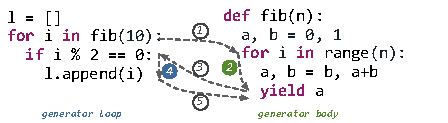
\includegraphics[scale=1.5]{figures/ch4-gen-exec-order}
\caption{Program execution order of a generator loop}
\label{fig:ch4-gen-exec-order}
\end{figure}

Figure~\ref{fig:ch4-gen-exec-order} shows a generator loop (left) that collects even numbers among the first ten Fibonacci numbers generated by \texttt{fib} (right) into the list \texttt{l}.
For each iteration in the loop, the program performs the following steps:

\begin{enumerate}
\item Call \texttt{\_\_next\_\_} on the generator and resume execution.

\item Perform another iteration in the for \texttt{range} loop to compute the next Fibonacci number.

\item Return the value of \texttt{a} to the caller and assign it to \texttt{i}.

\item Execute the body of the generator loop.

\item Return to the loop header and continue with the next iteration.
\end{enumerate}

Among those steps listed above, only step two and four perform the actual computation.
Steps one and three are generator specific resume and suspend steps.
They involve calling a function, resuming the generator AST to the previous state and returning the next value back to the caller.
Those generator specific steps add high overhead to the real work in the generator loop.

The most common and effective technique for optimizing function calls is to inline callees into callers.
However, traditional function inlining does not work for generators.
The desugared generator loop (similar to the one shown in Figure~\ref{fig:ch4-iterate-on-generator-code}) includes two calls: one to the generator function \texttt{fib} and another one to the \texttt{\_\_next\_\_} method.
The call to \texttt{fib} simply returns a generator object during loop setup, and is not performance critical.
Inlining the call to \texttt{\_\_next\_\_} requires special handling of \emph{yield}s rather than treating them as simple returns.
An ideal solution should handle both calls at the same time, while still preserving semantics.

Observe that the generator loop always calls \texttt{\_\_next\_\_} on the generator unless it terminates.
If the generator loop body was empty, we can replace the loop with the generator body of \texttt{fib} and still preserve semantics.
Furthermore, assuming the above mentioned replacement is in-place, for the non-empty loop body case, we can replace each yield statement with the generator loop body.
Figure~\ref{fig:ch4-peeling-trans} illustrates this transformation.
The solid arrow depicts the generator loop replacement that ``inlines'' the generator body.
The dashed arrow shows the yield replacement that combines the generator code and the caller code.

Figure~\ref{fig:ch4-fib-peeled} shows the pseudo-code of the transformed program.
We combine the generator body and the loop body in the same context.
The original call to the generator function \texttt{fib} translates to the assignment to \texttt{n} which sets up the initial state of the following generator body.
The generator body replaces the original generator loop.
We simplify the yield statement to a single assignment.
The assignment transfers the value of \texttt{a} from the generator body to the following loop body.
The loop body in turn consumes the ``yielded'' value of \texttt{i}.

\begin{figure}[!t]
\centering
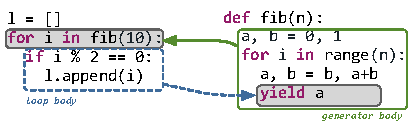
\includegraphics[scale=1.5]{figures/ch4-peeling-generator-call}
\caption{Peeling transformation}
\label{fig:ch4-peeling-trans}
\end{figure}

\begin{figure}[!t]
\centering
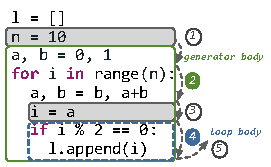
\includegraphics[scale=1.5]{figures/ch4-fib-peeled}
\caption{Transformed generator loop}
\label{fig:ch4-fib-peeled}
\end{figure}

The transformation peels off the generator loop, and removes both calls, to \texttt{fib} and \texttt{\_\_next\_\_}.
The optimized program does not create a generator object.
It eliminates the step one and simplifies the step three shown in Figure~\ref{fig:ch4-gen-exec-order}.
These two steps do not contribute to the real computation.
The numbers on the right of Figure~\ref{fig:ch4-fib-peeled} denote the corresponding execution steps of the original generator loop shown in Figure~\ref{fig:ch4-gen-exec-order}.
The two assignments preceding the transformed generator body and the loop body (grayed in Figure~\ref{fig:ch4-fib-peeled}) preserve the correct data flow into and out of the generator code.

We simplified the pseudo code shown in Figure~\ref{fig:ch4-fib-peeled} for clarity.
Our transformation is not limited to the case where the call to the generator function happens at the beginning of the consuming loop.
If the creation of the generator object happens before the loop, we apply the same transformation that combines the generator body with the loop body.
We explain the actual AST transformation in more detail in Section~\ref{sec:ch4-ast-transformation}.

\subsection{Peeling AST Transformations}
\label{sec:ch4-ast-transformation}

\begin{figure*}
\centering
\subfigure[AST transformation]{
	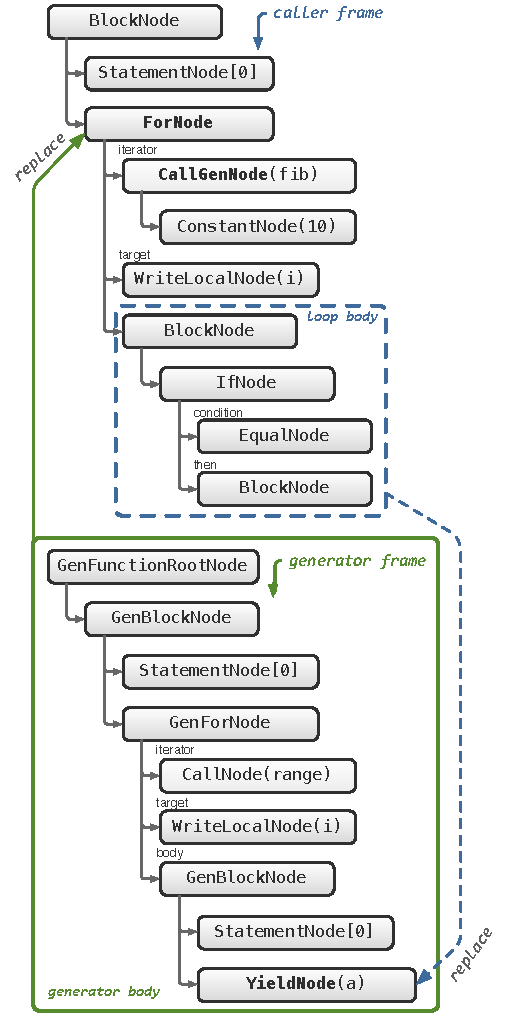
\includegraphics[scale=.82]{figures/ch4-ast-before-peeling}
	\label{fig:ch4-ast-before-peeling}
}
\subfigure[Transformed generator loop AST]{
	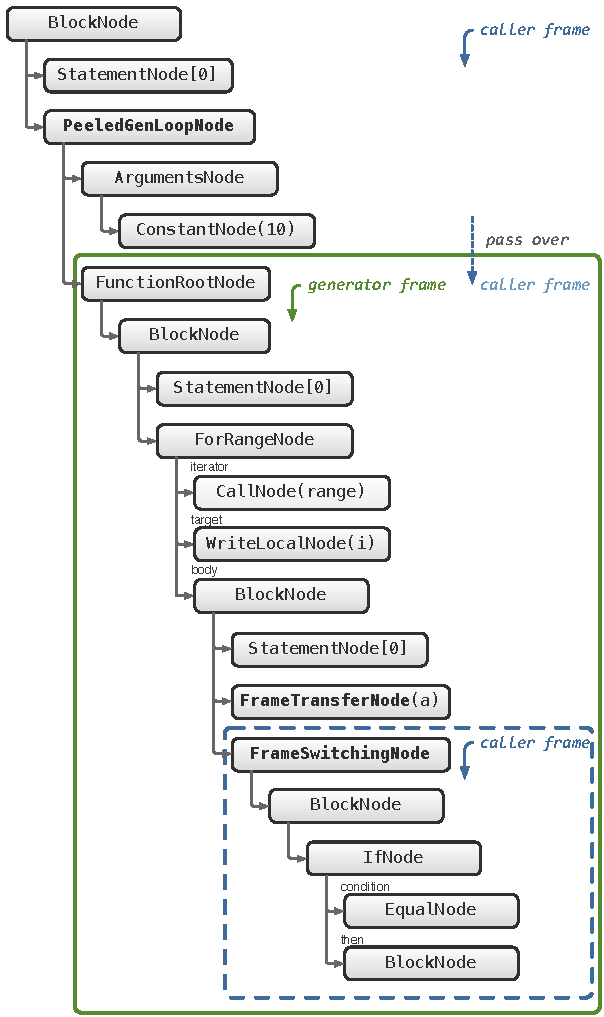
\includegraphics[scale=.82]{figures/ch4-peeled-ast}
	\label{fig:ch4-peeled-ast}
}
\caption{Peeling AST transformation}
\label{fig:ch4-ast-transformation}
\end{figure*}

Figure~\ref{fig:ch4-ast-before-peeling} shows the AST transformation of our Fibonacci example.
The upper half of the figure shows the AST of the generator loop.
The AST contains a \texttt{CallGenNode} that calls the generator function \texttt{fib}, and returns a generator object to its parent node.
The parent \texttt{ForNode} representing the for loop then iterates over the generator.
The lower half of the figure shows the AST of the generator function \texttt{fib}.
Note that the generator body AST uses generator control nodes and includes the \texttt{YieldNode} that returns the next Fibonacci number to the caller.

The figure also illustrates the two-step peeling AST transformation.
First we replace the \texttt{ForNode} that iterates over the generator with the AST of the generator body.
Second, we clone the AST of the loop body and use it to replace the \texttt{YieldNode} in the generator body.
Figure~\ref{fig:ch4-peeled-ast} shows the result of the transformation.
We use a \texttt{PeeledGenLoopNode} to guard the transformed generator body.
The \texttt{PeeledGenLoopNode} receives the arguments from the \texttt{ArgumentsNode} and passes them the transformed generator body.
The \texttt{FrameTransferNode} transfers the Fibonacci number stored in the variable \texttt{a} to the following loop body (equivalent to step three in Figure~\ref{fig:ch4-fib-peeled}).
The transformed loop body in turn consumes the ``yielded'' number.

ZipPy implements a number of different versions of \texttt{PeeledGenLoopNode} to handle different loop setups.
For instance, a generator loop could consume an incoming generator object without calling the generator function at the beginning of the loop.
The transformed \texttt{PeeledGenLoopNode} in this case guards against the actual call target wrapped by the incoming generator object and receives the arguments from the generator object.

\subsection{Polymorphism and Deoptimization}
\label{sec:ch4-polymorphic-and-deopt}

ZipPy handles polymorphic operations by forming a chain of specialized nodes with each node implementing a more efficient version of the operation for a particular operand type.
The interpreter then dispatches execution to the desired node depending on the actual type of the operand.
Like other operations in Python, the type of the iterator coming into a loop can change at runtime.
A loop that iterates over multiple types of iterators is a polymorphic loop.

\begin{figure}
\centering
\subfigure[Monomorphic]{
	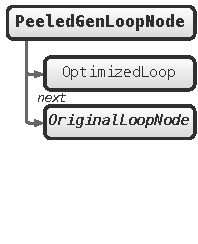
\includegraphics[scale=1.15]{figures/ch4-ast-peeled-mono}
	\label{fig:ch4-ast-peeled-mono}
}
\subfigure[Polymorphic]{
	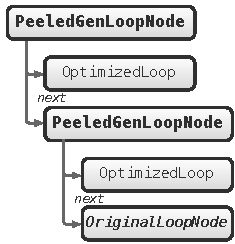
\includegraphics[scale=1.15]{figures/ch4-ast-peeled-poly}
	\label{fig:ch4-ast-peeled-poly}
}
\subfigure[Deoptimized]{
	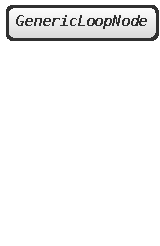
\includegraphics[scale=1.15]{figures/ch4-ast-peeled-deopt}
	\label{fig:ch4-ast-peeled-deopt}
}
\caption{Handling of polymorphic generator loop}
\label{fig:ch4-peeling-polymorphic}
\end{figure}

Generator peeling is a loop specialization technique that targets generators, a particular kind of iterators.
ZipPy handles polymorphic loops by forming a chain of specialized loop nodes including \texttt{PeeledGenLoopNode}s.
A \texttt{PeeledGenLoopNode} checks the actual call target of the incoming iterator before it executes the optimized loop.
As shown in Figure~\ref{fig:ch4-peeling-polymorphic}, if the target changes, then the execution falls through to the original loop node.
ZipPy is able to apply an additional level of the generator peeling transformation for the new iterator type if it happens to be a generator as well.

However, forming a polymorphic chain that is too deep could lead to code explosion.
If the depth of the chain goes beyond a pre-defined threshold, ZipPy stops optimizing the loop and replaces the entire chain with a generic loop node.
The generic loop node is capable of handling all types of incoming iterators but with limited performance benefit.

\subsection{Frames and Control Flow Handling}
\label{sec:ch4-frame-and-control}

The AST of the optimized generator loop combines nodes from two different functions and therefore accesses two different frame objects.
Programmers can use non-local control flows such as \texttt{break}s or \texttt{continue}s in a generator loop body.
We explain how to handle frames and such control flows in the rest of this section.

\subsubsection*{Frame Switching}

% two frames in the fig
The transformed AST illustrated in Figure~\ref{fig:ch4-peeled-ast} accesses two frames: the caller frame and the generator frame.
Figure~\ref{fig:ch4-two-frames} shows the layouts of the two frames.
The nodes belonging to the caller function read from and write to the caller frame to access its local variables.
The generator body nodes do so through the generator frame.
The \texttt{PeeledGenLoopNode} allocates the generator frame and passes it to the dominated generator body.
To enable caller frame access in the deeply nested loop body, the node also passes over the caller frame.
Therefore, in the sub-tree dominated by the \texttt{PeeledGenLoopNode}, both frames are accessible.

\begin{figure}[!ht]
\centering
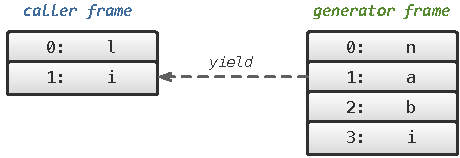
\includegraphics[scale=1.2]{figures/ch4-two-frames}
\caption{The caller and generator frame objects of the Fibonacci example}
\label{fig:ch4-two-frames}
\end{figure}

% passing caller over and switches between two frames
Although keeping both frames alive and accessible, the interpreter picks one frame object as the current frame and retains the other one as the background frame.
It passes the current frame to every \texttt{execute} method of the AST nodes as an argument for faster access.
The current frame stores a reference to the background frame.
The accesses to the background frame require one more level of indirection.

In the generator body shown in Figure~\ref{fig:ch4-peeled-ast}, the interpreter sets the generator frame as the current frame.
The \texttt{FrameTransferNode} propagates the values of \texttt{a} in the generator frame to \texttt{i} in the caller frame.
This value propagation corresponds to step 3 in Figure~\ref{fig:ch4-gen-exec-order} and Figure~\ref{fig:ch4-fib-peeled}.
The following \texttt{FrameSwitchingNode} swaps the positions of the two frames and passes the caller frame as the current frame to the dominated loop body.

% truffle remove frame allocation.
Truffle's underlying JIT compiler optimizes frame accesses.
It eliminates frame allocations as long as references to the frame object are not stored on the heap.
A generator stores its execution state by keeping a frame object reference on the heap.
Therefore, the generator AST introduced in Section~\ref{sec:ch4-generator-ast} prevents this frame optimization.
After generator peeling, however, the program does not create and iterate over generators.
It is not necessary to adopt generator control nodes in the ``inlined'' generator body and store frame object references on the heap.
As a result, the compiler can successfully optimize frame accesses in the transformed generator loop regardless of the number of frames.

For generator functions containing multiple yields, we apply the same transformation to each \texttt{YieldNode}.
The resulting AST contains more than one loop body, hence multiple \texttt{FrameSwitchingNode}s.
We rely on the control-flow optimizations of the underlying compiler to minimize the cost of this replication.

Merging both frames could also guarantee correct frame accesses in the transformed AST.
However, this approach is more complicated.
Merging frames combines the allocations of both frames, which requires redirecting all frame accesses to the combined frame.
Upon deoptimization, we need to undo the merge and redirect all frame accesses back to their separate frames.
This process become more complex for the nested generator loop scenario which we explain more in Section~\ref{sec:ch4-multilevel-peeling}.
Since the underlying compiler is able to optimize multiple frame objects, merging frames does not produce faster code.

\subsubsection*{Breaks and Continues}

\begin{figure}
\centering
\subfigure[Break handling]{
	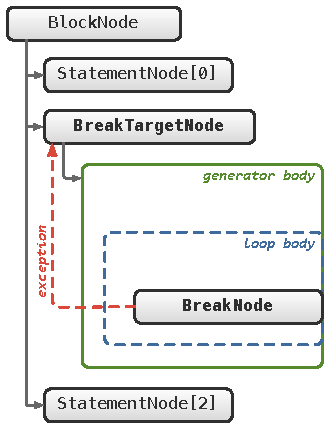
\includegraphics[scale=1.1]{figures/ch4-break-handling}
	\label{fig:ch4-break-handling}
}
\subfigure[Continue handling]{
	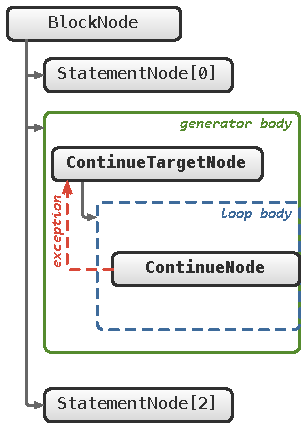
\includegraphics[scale=1.1]{figures/ch4-continue-handling}
	\label{fig:ch4-continue-handling}
}
\caption{Complex control flow handling}
\label{fig:ch4-break-and-continue}
\end{figure}

ZipPy implements break and continue statements using Java exceptions.
A \texttt{BreakNode} throws a break exception, and then a parent node catches the exception.
The control flow exception skips all the nodes between the throwing node and the catching node.
The location of the catch clause determines what the exception can skip.
Figure~\ref{fig:ch4-gen-while-node-code} shows the catch clause in a \texttt{GenWhileNode}.
The node catches the break exception after the while loop, hence the exception breaks the loop.
Similarly, a continue exception caught in the loop body quits the current iteration and continues with the next iteration.
There are no labeled break or continue statements in Python.
Thus, a control flow exception does not go beyond its enclosing loop.
Furthermore, we can extract the exception catch clauses to dedicated nodes to construct more complicated control structures.

A generator loop body may contain break or continue statements that target the generator loop.
Generator peeling replaces the generator loop and embeds the loop body inside the generator body.
To properly handle breaks in the loop body, we interpose a \texttt{BreakTargetNode} between the caller and the generator body as shown in Figure~\ref{fig:ch4-break-handling}.
The nested \texttt{BreakNode} throws a dedicated break exception to skip the generator body, before it reaches the \texttt{BreakTargetNode}.
After catching the exception, the \texttt{BreakTargetNode} returns to its parent and skips the rest of the generator loop.
We handle continues by interposing a \texttt{ContinueTargetNode} between the loop body and the generator body (see Figure~\ref{fig:ch4-continue-handling}).
A continue exception skips the rest of the nodes in the loop body and returns execution to the generator body.
This control flow is equivalent to what a continue does in the original generator loop, that is resuming the generator execution from the statement after the last yield.

The above mentioned interposition is only necessary when the optimized loop body contains break or continue statements.
As we explained in Section~\ref{sec:ch4-ast-of-gen-func}, the underlying compiler optimizes control-flow exceptions into direct jumps.
Therefore, the exception-based control handling has no negative impact on peak performance.

\subsection{Implicit Generator Loops}

\begin{figure}[th]
\centering
\subfigure[Original]{
	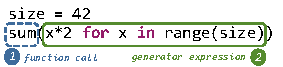
\includegraphics[scale=1.5]{figures/ch4-implicit-orig}
	\label{fig:ch4-implicit-orig}
}

\subfigure[Inlined]{
	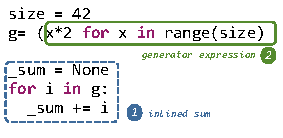
\includegraphics[scale=1.5]{figures/ch4-implicit-inlined}
	\label{fig:ch4-implicit-inlined}
}

\subfigure[Desugared]{
	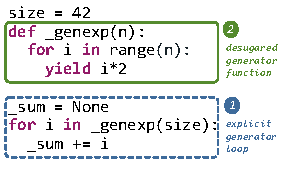
\includegraphics[scale=1.5]{figures/ch4-implicit-desugared}
	\label{fig:ch4-implicit-desugared}
}
\caption{Implicit generator loop transformation}
\label{fig:ch4-implicit-gen-loop}
\end{figure}

An implicit generator loop consists of a generator expression that produces a generator, and a function call that consumes the generator.
ZipPy applies additional transformation on implicit generator loops to enable further optimizations such as generator peeling.

Figure~\ref{fig:ch4-implicit-gen-loop} illustrates this two-step process.
First, we inline the function \texttt{sum} to expose the loop that consumes the generator (see Figure~\ref{fig:ch4-implicit-inlined}).
The inlining step triggers an escape analysis of all the generator expressions in the current scope.
If our analysis finds a generator expression such that the generator it produces does not escape the current scope and
a generator loop that consumes the produced generator exists, ZipPy desugars the expression to a generator function (see Figure~\ref{fig:ch4-implicit-desugared}).
Note that the desugared generator function redirects the references to the enclosing scope to the argument accesses in the local scope.
This redirection eliminates non-local variables in the generator expression and allows the compiler optimization for the enclosing frame.
The desugaring also replaces the generator reference in the inlined loop to a function call.
The transformation exposes the explicit generator loop that we can optimize using generator peeling.

One obstacle when optimizing an implicit generator loop is that the function consuming the generator can be a Python built-in function.
Programmers can use any built-in function that accepts iterable arguments in an implicit generator loop.
Table~\ref{tab:ch4-builtins} lists all the Python 3 built-in functions that accept iterables and divides them into three different categories:

\begin{table}[!ht]
  \begin{center}
    \begin{tabular}{ c c c }
      \toprule
      1. Implement in                & 2. Synthesize to loop & 3. No loop \\
      Python                         &                       & \\
      \midrule
      \texttt{all}, \texttt{any}     & \texttt{bytes}        & \texttt{iter} \\
      \texttt{bytearray}             & \texttt{dict}         & \texttt{next} \\
      \texttt{enumerate}             & \texttt{frozenset}    &               \\
      \texttt{filter}, \texttt{list} & \texttt{set}          &               \\
      \texttt{map}, \texttt{max}     & \texttt{tuple}        &               \\
      \texttt{min}, \texttt{sorted}  &                       &               \\
      \texttt{sum}, \texttt{zip}     &                       &               \\
      \bottomrule
    \end{tabular}
    \nocaptionrule{}
    \caption{Python Built-in functions that accept iterables}
    \label{tab:ch4-builtins}
  \end{center}
\end{table}

\begin{enumerate}

\item \textbf{Implement in Python}:
Convenience functions that one can write in pure Python.
ZipPy implements these functions using Python code.
They share the same inlining approach with user defined functions.

\item \textbf{Synthesize to loop}:
Constructors of immutable data types in Python.
Cannot be written in pure Python without exposing internal data representations of the language runtime.
The current solution is to speculatively intrinsify the built-in call by replacing the call node with a synthesized AST.
The synthesized AST contains the generator loop and constructs the desired data type.
The intrinsified call site exposes the generator loop and enjoys the same peeling optimization.

\item \textbf{No loop}:
Contains no loop.
We exclude them from the optimization.

\end{enumerate}

\subsection{Multi-level Generator Peeling}
\label{sec:ch4-multilevel-peeling}

ZipPy relies on the tiered execution model of the underlying framework.
It starts executing a Python program in interpretation mode.
The interpreter collects runtime information and inlines function calls that are hot.
We apply function inlining using an inlining budget.
This budget helps to prevent code explosions caused by inlining too many calls or too big a callee.
We perform generator peeling when a generator function call becomes hot, and possibly bail out if the transformation did not succeed.
Generator peeling shares its budget with function inlining.
If a generator peeling transformation is going to overrun the inlining budget, ZipPy aborts the transformation.
After exhausting all possible inlining and peeling opportunities, Truffle compiles the entire AST into machine code.
All subsequent calls to the compiled function execute at peak performance.

\begin{figure}
\centering
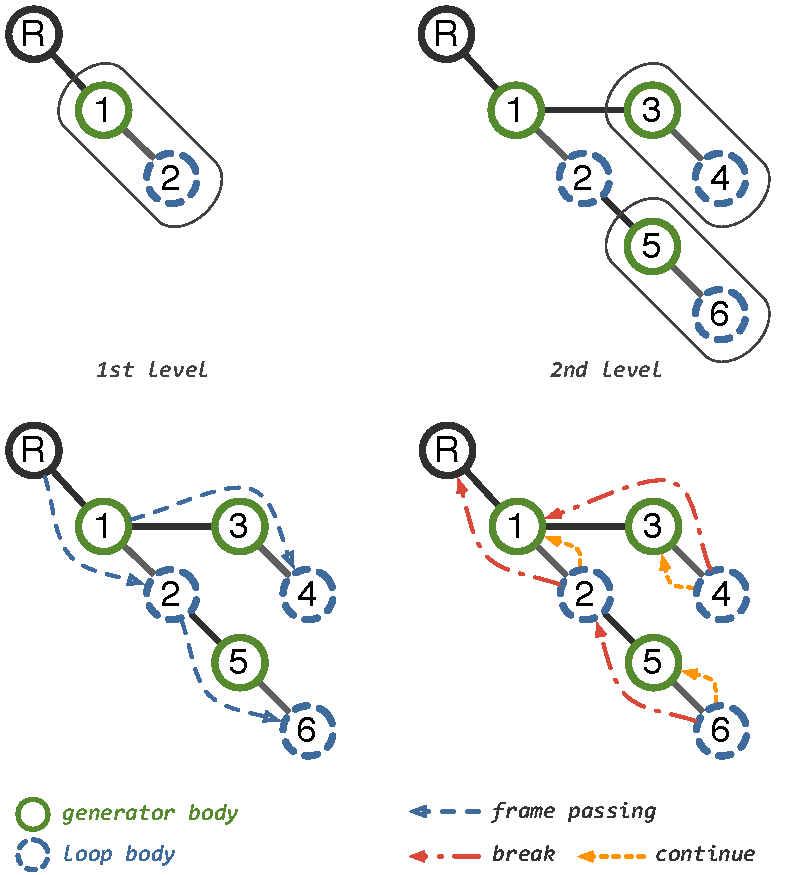
\includegraphics[scale=.9]{figures/ch4-multilevel-peeling}
\caption{Multi-level generator peeling}
\label{fig:ch4-multilevel-peeling}
\end{figure}

An optimized generator loop might include another generator loop.
We call these cases nested generator loops.
Python programs can contain arbitrary levels of nested generator loops.
Our optimization is capable of handling multiple levels of nested generator loops by iteratively peeling one loop layer at a time.
It requires minimal modifications to our existing algorithms to handle this scenario.

Figure~\ref{fig:ch4-multilevel-peeling} shows the AST of three nested generator loops after peeling transformations.
In a simple case, an optimized generator loop consists of two parts: the inlined generator body and the embedded loop body.
To illustrate the relationships between these two program regions, we simplify the structure of the AST by using one node for each program region.
A numbered solid circle denotes a generator body, and a numbered dashed circle denotes a loop body.
An ``inlined'' generator body node is always associated with a loop body node as its immediate child.
As shown in Figure~\ref{fig:ch4-multilevel-peeling}, the first level peeling results in node one being the generator body and node two being the loop body.
The second level peeling includes two optimized generator loops with nodes three and four extended from the generator body and nodes five and six extended from the loop body.
Note that at any level in the tree, a next level peeling can either extend from the generator body or the loop body of the current level.
More complicated cases recursively repeat the same tree structure as shown in Figure~\ref{fig:ch4-multilevel-peeling}.
Therefore, a working solution for the shown tree structure automatically extends to more complicated cases.

% rules in the tree
The tree shown in the figure adheres to the following rules:
Since it is a tree, every node only has one parent except the root node.
Every solid node has an associated dashed node as its child but possibly not the only child.
Every dashed node has an associated solid node as its only parent.
Every dashed node must have one and only one grandparent.

The arrows in Figure~\ref{fig:ch4-multilevel-peeling} depict the desired frame and control-flow handling.
Every dashed node receives two frames: one from its parent and another one from its grandparent.
Since every dashed node has a unique parent and a unique grandparent, there it no ambiguity on which two frames it receives.
A \texttt{continue} returns from a dashed node to its associated solid node.
Since the associated solid node is its only parent, no node can intercept this control-flow.
Our existing algorithms therefore automatically cover frame handling and continue statements for nested generator loops.

Break statements are more complicated.
A \texttt{break} returns from a dashed node to its grandparent.
However, its solid parent node may be the break target of another node and intercept the break exception.
For instance, node one in the figure might catch the break exception thrown in node two or node four.
This ambiguity may cause an incorrect break from node two.
To resolve this issue, we need to label the overlapping break exceptions to filter out undesired ones.
Since it is rare to have two nested generator loops that both use breaks, we consider this scenario as a corner case.

In summary, our peeling transformation is able to handle arbitrary levels of nested generator loops.
